% Appendix A

\chapter{Datos Obtenidos} % Main appendix title

\label{AppendA} % For referencing this appendix elsewhere, use \ref{AppendixA}
\section{Precisión de entrenamiento}
\begin{figure}[H]
	\begin{centering}
		\subfloat[fig 1]{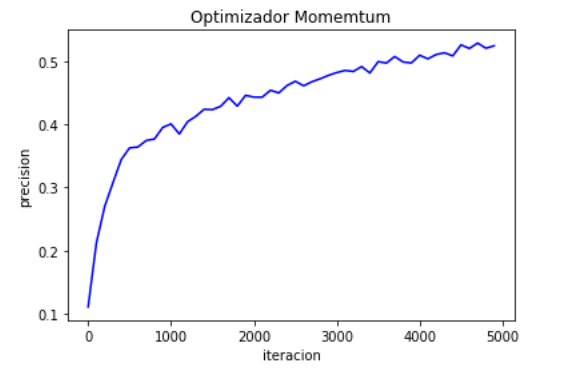
\includegraphics[width=0.45\textwidth]{Figures/momemtum5000.png}} 
		\subfloat[fig 2]{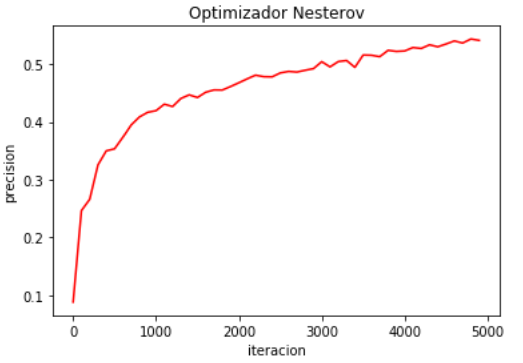
\includegraphics[width=0.45\textwidth]{Figures/nesterov5000.png}}\\
		\subfloat[fig 3]{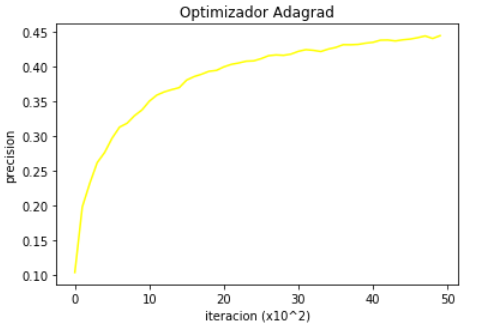
\includegraphics[width=0.45\textwidth]{Figures/adagrad5000.png}}
		\subfloat[fig 3]{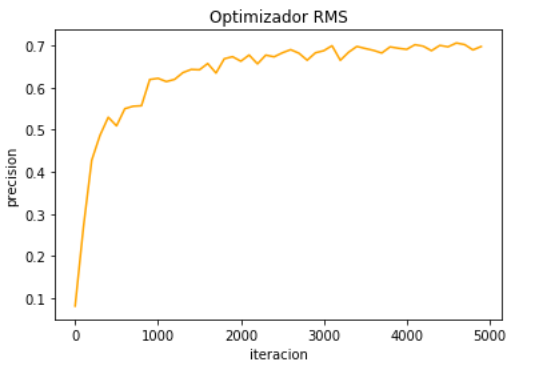
\includegraphics[width=0.45\textwidth]{Figures/rms5000.png}}\\
		\subfloat[fig 4]{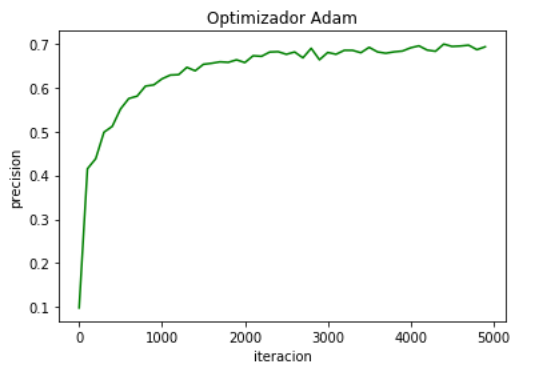
\includegraphics[width=0.5\textwidth]{Figures/adam5000.png}} 
		\caption{optmizadores 5000 epochs \\ Fuente :{\textit{Fuente Propia}}}
		\caption{Estructura de la imagen de entrada \\ Fuente:  \textit{Fuente Propia}}
		\label{some example}
	\end{centering}

\end{figure}


\begin{figure}[H]
	\begin{centering}
		\subfloat[fig 1]{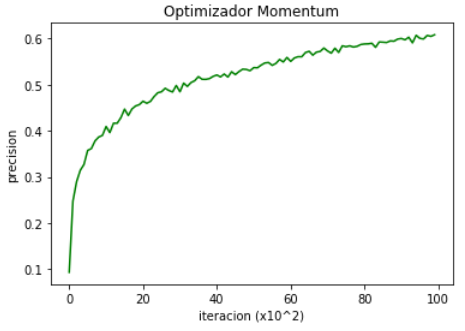
\includegraphics[width=0.55\textwidth]{Figures/momemtum10000.png}} 
		\subfloat[fig 2]{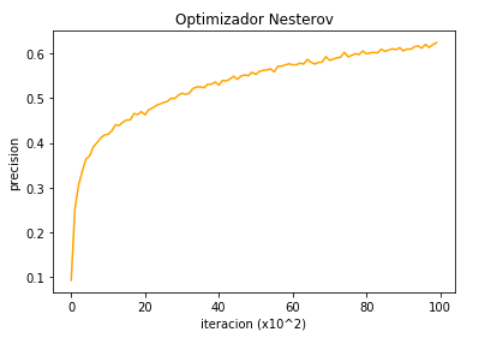
\includegraphics[width=0.55\textwidth]{Figures/nesterov10000.png}}\\
		\subfloat[fig 3]{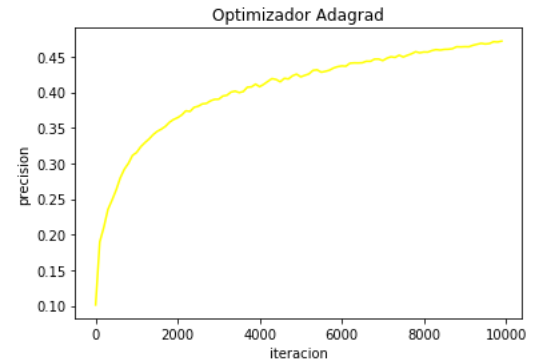
\includegraphics[width=0.55\textwidth]{Figures/adagrad10000.png}}
		\subfloat[fig 3]{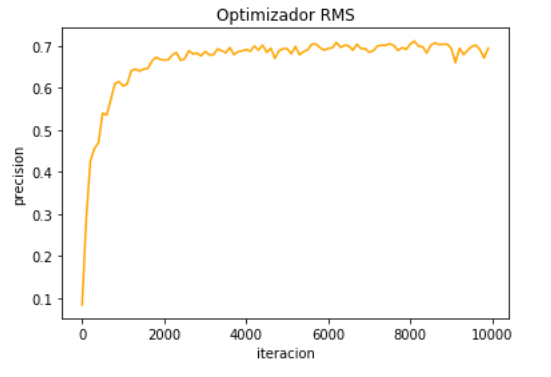
\includegraphics[width=0.55\textwidth]{Figures/rms10000.png}}\\
		\subfloat[fig 4]{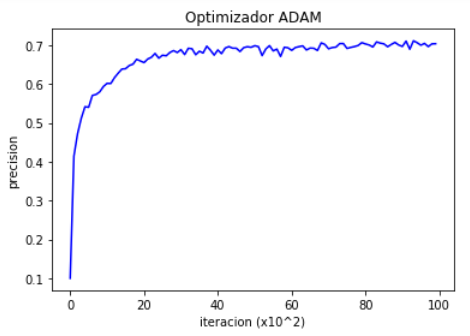
\includegraphics[width=0.6\textwidth]{Figures/adam10000.png}} 
		\caption{optmizadores 10000 epochs\\ Fuente:  \textit{Fuente Propia}}
		\label{some example}
	\end{centering}
	
\end{figure}

\begin{figure}[H]
	\begin{centering}
		\subfloat[fig 1]{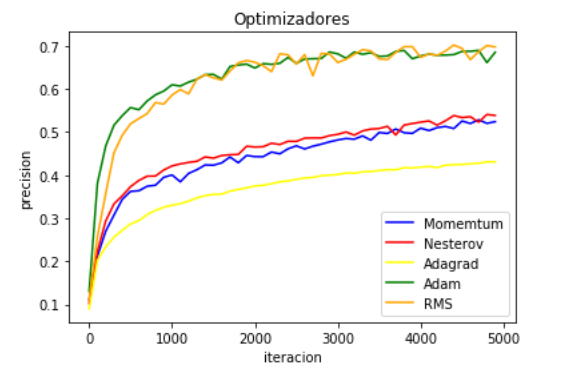
\includegraphics[width=0.8\textwidth]{Figures/optimizadoresv25000.png}} 
		\caption{Comparación de optimizadores para 5000 epochs\\ Fuente:  \textit{Fuente Propia}}
		\label{some example}
	\end{centering}
	
\end{figure}

\begin{figure}[H]
	\begin{centering}
		\subfloat[fig 1]{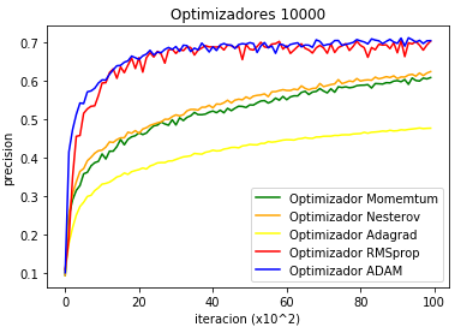
\includegraphics[width=0.8\textwidth]{Figures/optimizadores10000.png}} 
		\caption{Comparación de optimizadores para 10000 epochs\\ Fuente:  \textit{Fuente Propia}}
		\label{some example}
	\end{centering}
	
\end{figure}

\section{Función de Costo}
\begin{figure}[H]
	\begin{centering}
		\subfloat[fig 1]{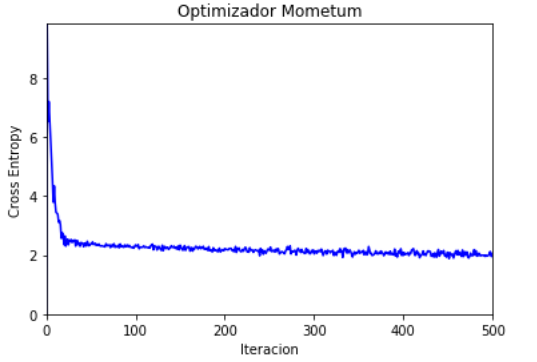
\includegraphics[width=0.5\textwidth]{Figures/momemtumcross5000.png}} 
		\subfloat[fig 2]{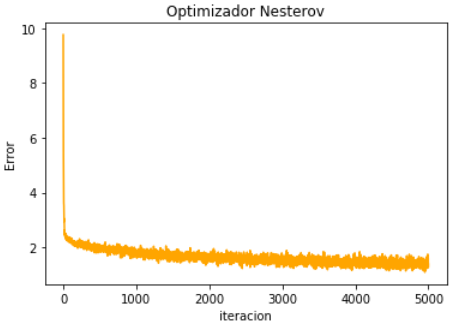
\includegraphics[width=0.5\textwidth]{Figures/nesterovcross5000.png}}\\
		\subfloat[fig 3]{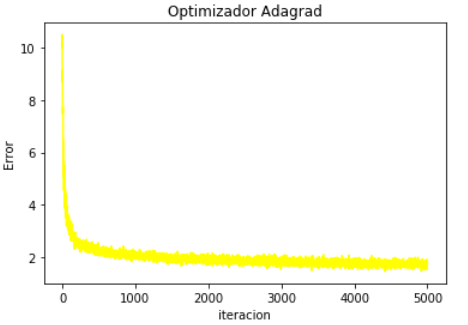
\includegraphics[width=0.5\textwidth]{Figures/adagradcross5000.png}}
		\subfloat[fig 3]{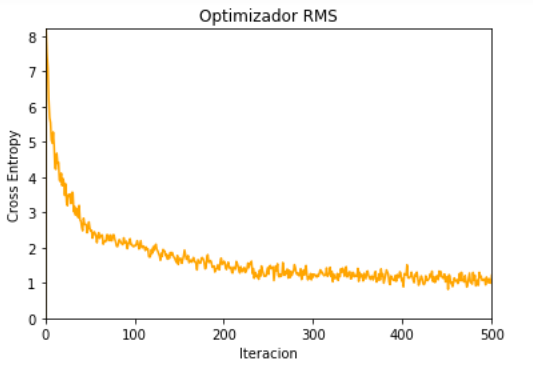
\includegraphics[width=0.5\textwidth]{Figures/rmscross5000.png}}\\
		\subfloat[fig 4]{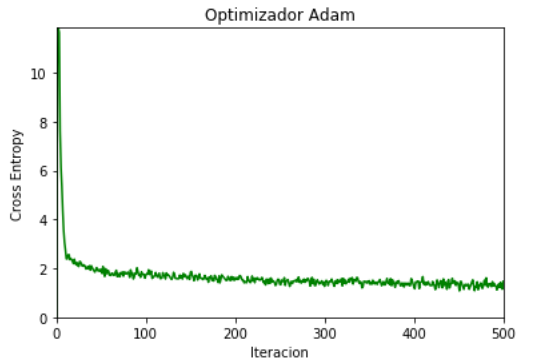
\includegraphics[width=0.5\textwidth]{Figures/adamcross5000.png}} 
		\caption{función de costo de optimizadores\\ Fuente:  \textit{Fuente Propia}}
		\label{some}
	\end{centering}
	
\end{figure}

\begin{figure}[H]
	\begin{centering}
		\subfloat[fig 1]{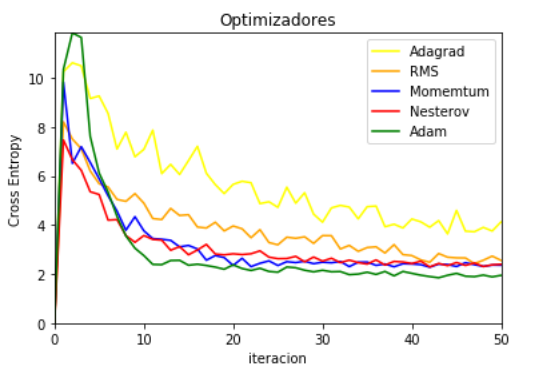
\includegraphics[width=0.8\textwidth]{Figures/cross500050.png}} 
		\caption{Comparación de las funciones de costo rango 0-50\\ Fuente:  \textit{Fuente Propia}}
		\label{some example}
	\end{centering}
	
\end{figure}

\begin{figure}[H]
	\begin{centering}
		\subfloat[fig 1]{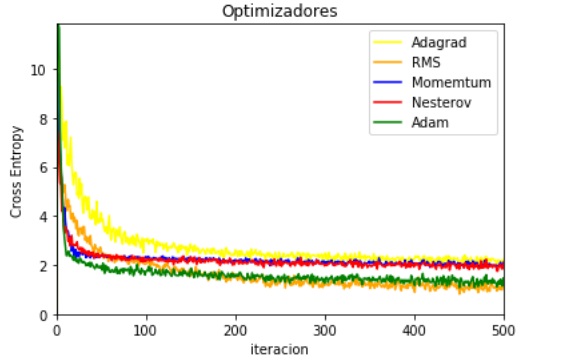
\includegraphics[width=0.8\textwidth]{Figures/cross5000500.png}} 
		\caption{Comparación de las funciones de costo rango 0-500\\ Fuente:  \textit{Fuente Propia}}
		\label{some example}
	\end{centering}
	
\end{figure}